\newcommand{\assignmentControl}{\textit{assignment-control}}
\newcommand{\propagationControl}{\textit{propagation-control}}
\subsection{Labeling policies}
\label{sec:administrative-model}
 


 
 In this section, we discuss specification of labeling policies for the operational model given in Section \ref{sec:operational-model}. We broadly categorize the policies used in the operational model into specification of authorization policies and assignment of security-label values or labeling policies. Policy scope of the operational model is schematically shown in Figure \ref{fig:administration-scope}. Here, we focus on the later type of policies.
 
   
 	\begin{figure} [t]
 		\centering
 		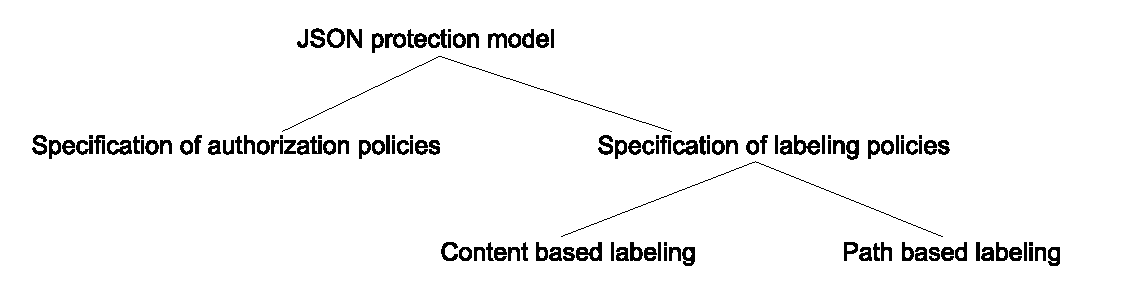
\includegraphics[width=1\textwidth]{NSS16/administration-scope}
 		\caption{Policy scope}
 		\label{fig:administration-scope}
 	\end{figure}
 
 
 We specify two different approaches to assign security-label values to elements in a JSON document, viz. content-based and  path-based. These approaches are fundamentally different in how a JSON element is specified. While a path is described starting from the root node of the tree, content is specified starting from the leaf nodes of the tree. These two contrasting approaches offer flexibility in assignments and propagation of security-label values.
 
 %The scope of administration is shown in Figure \ref{fig:administration-scope}. We broadly categorize administrative scope into administration of authorization policies and assignment of security-label values. The former is related to administration of enumerated authorization policy ABAC models which is an interesting problem of its own. This paper only discusses assignments of security-label values in the context of JSON documents.
 
 \subsubsection{Control on labeling policies}
 
 

For specification of labeling policies, we define two types of restriction that control assignments and propagations of \textit{security-label} values. In the first type, we restrict how security-label values are selected and assigned on tree nodes. We call this \assignmentControl{}. In the second type, we specify how assigned values are propagated along nodes in the tree. We call this \propagationControl{}. 
 
  	\begin{figure} [t]
 		\centering
 		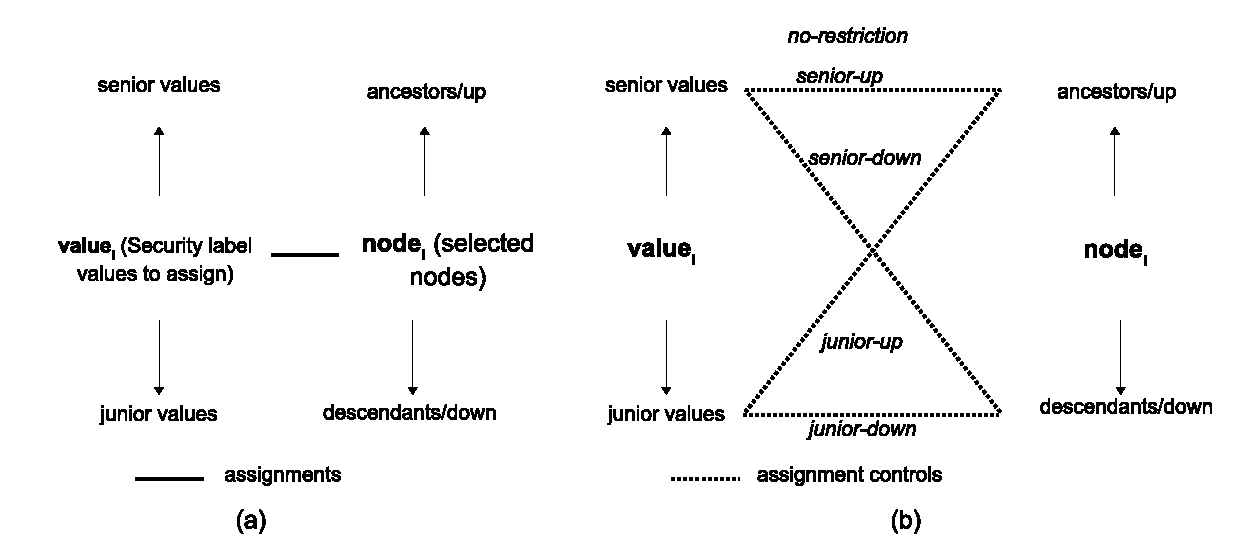
\includegraphics[width=1\textwidth]{NSS16/assignment-control}
 		\caption{Demonstration of (a) assignment of security label values and (b) assignment controls}
 		\label{fig:restriction-types}
 	\end{figure}
 
 
 The motivation of \assignmentControl{} is to restrict arbitrary assignments of security-label values. This enables administrators to restrict future assignments after some assignments have been carried out.  These controls are specified during the assignments. If any attempting assignment does not comply with \assignmentControl{}s of existing assignments, it will be discarded. We define five possible options for \assignmentControl{} as \textit{no-restiction}, \textit{senior-up}, \textit{senior-down}, \textit{junior-up} and \textit{junior-down}. The type \textit{no-restriction} does not specify any restriction. If we assign a value $value_i$ in $node_i$, with \textit{senior-up} restriction, all up/ancestors of $node_i$ must be assigned values senior to $value_i$ possibly including $value_i$. In type \textit{senior-down} restriction, all down/descendants of $node_i$ must be assigned values senior to $value_i$ possibly including $value_i$.  Similarly, the types \textit{junior-up} and \textit{junior-down}, specify that ancestors and descendants of $node_i$ must be assigned  values junior to $value_i$, possibly including $value_i$.  Figure \ref{fig:restriction-types} schematically illustrates \assignmentControl{}. In Figure \ref{fig:propagation-option}, the node \textit{con-info} is assigned a value \textit{enterprise} with option \textit{junior-down} which regulates that its descendant nodes namely \{email, work-phone\} must be assigned values $enterprise$ or its juniors, in this case from the set \{enterprise, public\} (using security-label values given in Figure \ref{fig:operational-explanation}(b)). In the same figure, the node \textit{sen-info} is assigned value \textit{sensitive} with option \textit{senior-down} which mandates that its descendant nodes namely \{SSN, salary\} must be assigned values from \textit{sensitive} or its seniors in this case from the set \{sensitive\}.

%We define \textit{labeling options} to control how  security-label values are assigned to JSON elements. Possible options are \textit{unrestricted}, \textit{restricted-up} and \textit{restricted-down}. If unrestricted, a node can be assigned any security-label values allowed in the system. We can impose restriction for the assignments by using the options \textit{restricted-up} and/or \textit{restricted-down}. When we assign a value $V_i$  on a node $N_i$ (which is not unrestricted by existing assignments) with the option \textit{restricted-up}, it requires that all ancestor nodes (of $N_i$) must be assigned values equal or senior to $V_i$. Similarly, the option \textit{restricted-down} requires that all descendant nodes must be assigned a value equal or junior to $V_i$. Using these options, we can restrict the possible values that can be assigned to a node. Figure \ref{fig:propagation-option} explains how these options pose restriction for assignments of  security-label values on nodes in the tree. For example, 

   
 	\begin{figure} [t]
 		\centering
 		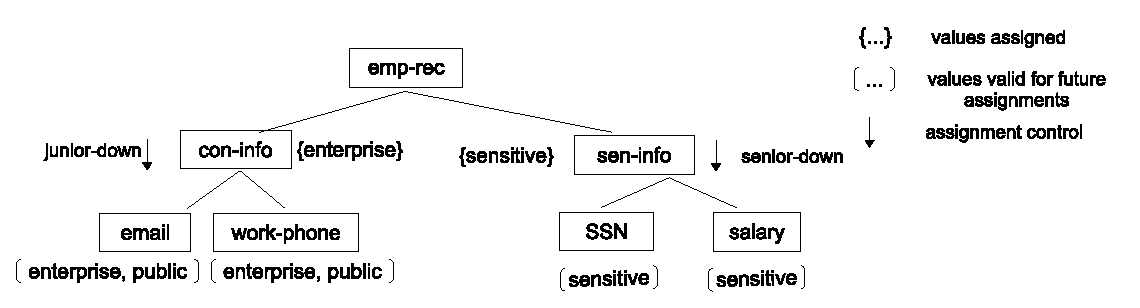
\includegraphics[width=1\textwidth]{NSS16/propagation-option}
 		\caption{Assignments with assignment controls}
 		\label{fig:propagation-option}
 	\end{figure}
% (considering security-label value hierarhcy given in Figure \ref{fig:operational-explanation})


 Once we assign security-label values on an element in a JSON tree, the value can be propagated to other elements in the tree. We define following  types for \propagationControl{} as \textit{no-prop},  \textit{one-level up}, \textit{one-level down},  \textit{cascading up} and \textit{cascading down}. Assigned values are not propagated in type \textit{no-prop}. From a node, assigned values are propagated to parent and all its siblings in the type \textit{one-level up}. Assigned values are propagated to all ancestor nodes in type \textit{cascading up}. Similarly, from a selected item, assigned values are propagated to direct children in type \textit{one-level down} and to all descendants in type \textit{cascading down}. % Propagation types are explained with an example in Figure \ref{fig:propagation-types}. 
 
%  
 	\begin{figure} [t]
 		\centering
 		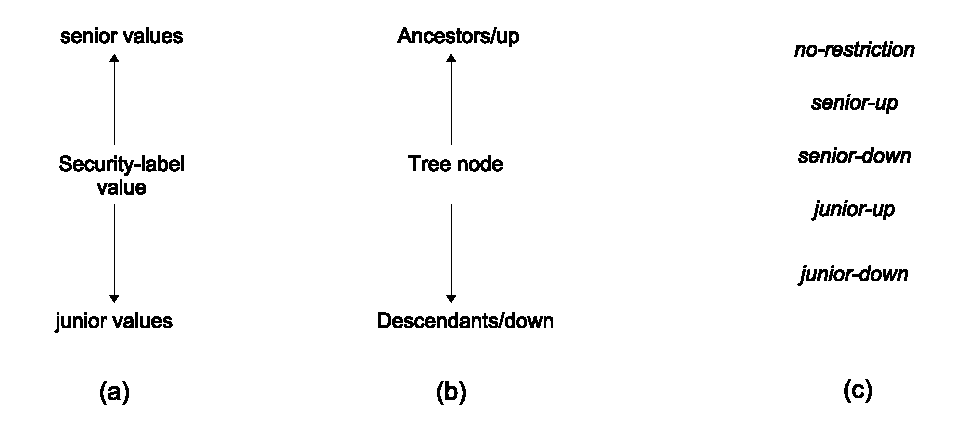
\includegraphics[width=1\textwidth]{propagation-types}
 		\caption{Example explaining propagation types}
 		\label{fig:propagation-types}
 	\end{figure}
 
 

\subsubsection{Content-based labeling}

  
 	\begin{figure} [t]
 		\centering
 		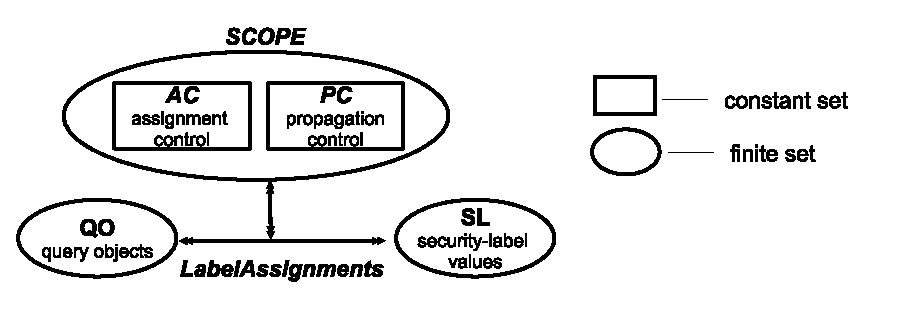
\includegraphics[width=1\textwidth]{NSS16/QO-based-labeling}
 		\caption{Content-based labeling model}
 		\label{fig:QO-based-labeling}
 	\end{figure}
  
\begin{table}[t]
	\centering
	\caption{Definition of content-based labeling} %\vspace*{3pt}
	\label{tab:QO-labeling-definition}			
	\begin{tabular}{|l|}
		\hline					
		\begin{tabular}{l}
			
				\multicolumn{1}{c}{\underline{\textit{I. Basic sets and relations}}}\\													
					
					- $QO$ (set of query objects). \\
					- $AC$ (assignment control) $AC$= \textit{\{no-restriction, senior-up, junior-up\}}.\\
					- $PC$ (propagation control) $PC = \{\noProp, \oneLevelUP, \cascadeUP\}$.\\

					- $SCOPE \subseteq  AC \times PC$\\
					- $SL$ (set of security-label values). \\
									
					\multicolumn{1}{c}{\underline{\textit{II. Assignments of security-label values}}}\\					
					- $\labelAssignment \subseteq QO \times SCOPE \times 2^{SL}$ \\ 

		\end{tabular}			
		 \\ \hline	
	\end{tabular}
	
\end{table}




This section shows how to assign security-label values by matching content and propagating the labels.

We adapt the concept of \textit{query object} available in MongoDB \cite{mongodb} which matches content in a JSON document. Query objects discover content starting from the \textit{value nodes} of the JSON tree. It accepts regular expression to find \textit{value nodes}  or \textit{key nodes} conveniently. MongoDB has built-in functions to express regular expressions and compare values matched by the regular expressions. 

A model to assign {security-label} values based on query objects is given in Figure \ref{fig:QO-based-labeling}. In the figure, $QO$ represents the set of all query objects and $SL$ is the set of {security-label} values. The set $AC$ represents \assignmentControl{} and $PC$ represents \propagationControl{} discussed earlier.  $AC$ and $PC$ together define labeling scopes. A labeling scope determines how values are assigned and propagated in the tree. As content is matched from the value/leaf nodes of the tree, we consider assignment and propagation control only for the ancestors of the matching nodes.

The formal definition of the model is given in Table \ref{tab:QO-labeling-definition}. Segment I of the table specify basic sets and relations. In Segment II, the relation \textit{ \labelAssignment{}} defines rules for assigning security-label values. An assignment rule is a triple of a query object to match content, a scope and a set of values to be assigned.  Section I of  Table \ref{tab:content-based-example} gives some examples of query objects and their interpretation in plain English.  Segment II of Table \ref{tab:content-based-example}, presents examples of assignment policies based on query objects.


\begin{table}[t]
	\centering
	\caption{ Examples of query objects and content-based labeling policies} %\vspace*{3pt}
	\label{tab:content-based-example}			
	\begin{tabular}{|l|}
		\hline					
		\begin{tabular}{l}
				\multicolumn{1}{c}{\underline{\textit{I. Query objects}}}\\										
				- ob1 = \{``email": \{ \$regex:``/.*@example.com/"\} \} (matches email addresses \\ \hfil from domain example.com)  \\
				- ob2 = \{ \$elemMatch: \{ \$regex: ``\reForEmail''  \} \} (matches any key having value \\ \hfil  corresponding to the  given regular expression) \\  
				- ob3 = \{\$elemMatch:\{ \$regex: ``\reSSN"\}, \$elemMatch: \{``\reCreditCard"\}\} \\ \hfil (matches all objects containing both social security and credit card number) \\
					
				\multicolumn{1}{c}{\underline{\textit{II. \labelAssignment}}}\\			
				- \labelAssignment = \{ (ob1, (no-prop, unrestricted), \{enterprise\}),   (ob2,\\ \hfil (no-prop, unrestricted),  \{enterprise\}), (ob3, (no-prop, restricted), \{ sensitive\} \}				\\
		\end{tabular}			
		 \\ \hline	
	\end{tabular}
	
\end{table}



 
 	\begin{figure}[t]
 		\centering
 		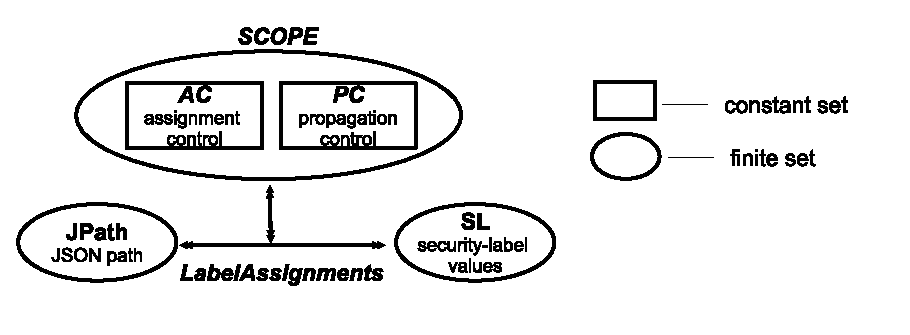
\includegraphics[width=1\textwidth]{NSS16/path-labeling-model}
 		\caption{Path-based labeling model}
 		\label{fig:path-based-labeling}
 	\end{figure}
 
\begin{table}[t]
	\centering
	\caption{Definition of Path-based labeling} %\vspace*{3pt}
	\label{tab:Path-labeling-definition}			
	\begin{tabular}{|l|}
		\hline					
		\begin{tabular}{l}
			
				\multicolumn{1}{c}{\underline{\textit{I. Basic sets and relations}}}\\	
					- $JPath$ (set of JSONPaths). \\
					- $AC$ (assignment control) $AC$= \textit{\{no-restriction, senior-down, junior-down\}}.\\
					- $PC$ (propagation control) $PC = \{\noProp, \oneLevelUP, \cascadeUP\}$.\\
					
					- $SCOPE \subseteq  AC \times PC$, relation to assign and propagate values.\\
					- $SL$ (set of security-label values). \\
									
					\multicolumn{1}{c}{\underline{\textit{II. Assignments of security-label values}}}\\					
					- $\labelAssignment \subseteq JPath \times SCOPE \times 2^{SL}$ (assign security-label values on \\ \hfill JSON elements matched and  propagate  values based on defined scope) \\ 

		\end{tabular}			
		 \\ \hline	
	\end{tabular}
	
\end{table}




\subsubsection{Path-based labeling}

In this section, we show how we assign security-label values by matching paths in the JSON tree and propagate them along the tree. 

We adapt \textit{JSONPath} \cite{JSONPath} to specify path-based labeling policies. This model is very similar to the content-based labeling model except we use JSONPath instead of query objects. While, query objects are matched starting from the leaf nodes, JSONPath specifies elements starting from the root node (or any node in case of relative path) and traverses towards leaf of the tree. As a result, this model apply assignment control and propagation control towards descendants of matching nodes.  The components of the model and its formal definition are given in Figure \ref{fig:path-based-labeling} and Table \ref{tab:Path-labeling-definition} respectively. Examples of JSON paths and path based labeling policies are presented in Segment I and II of Table \ref{tab:path-based-example}.


\begin{table}[t]
	\centering
	\caption{ Examples of JSONPath and path-based labeling policies} %\vspace*{3pt}
	\label{tab:path-based-example}			
	\begin{tabular}{|l|}
		\hline					
		\begin{tabular}{l}
				\multicolumn{1}{c}{\underline{\textit{I. JSONPaths}}}\\										
				- {path-to-email}=\$.{emp-rec.con-info.email}\\					
				- {path-to-salary}=\$.{emp-rec.sen-info.salary}\\
				\multicolumn{1}{c}{\underline{\textit{II. \labelAssignment}}}\\			
				- \labelAssignment = \{ (path-to-email, (no-prop, unrestricted), \{enterprise\}),  \\ \hfil (path-to-salary, (no-prop, unrestricted),  \{sensitive\}) \}				\\
		\end{tabular}			
		 \\ \hline	
	\end{tabular}
	
\end{table}



